%File: formatting-instruction.tex

\documentclass[letterpaper]{article}
\usepackage{aaai}
\usepackage{times}
\usepackage{helvet}
\usepackage{courier}
\usepackage{graphicx}
\usepackage{subcaption}
\frenchspacing
\setlength{\pdfpagewidth}{8.5in}
\setlength{\pdfpageheight}{11in}

%\documentclass{aamas2013}
\usepackage{amsfonts}
\usepackage{amsmath}
\usepackage{algorithmicx}
\usepackage{algpseudocode}
\usepackage{algorithm}

%\fontsize{24}{6}
%\selectfont

%\usepackage{draftwatermark}
%\SetWatermarkScale{1}
%\SetWatermarkLightness{.9}
%\SetWatermarkAngle{-45}
%\SetWatermarkText{DRAFT DRAFT DRAFT DRAFT}


%\usepackage[usenames]{color}
\DeclareMathOperator*{\argmin}{argmin}

%\makeatletter
%\let\@copyrightspace\relax
%\makeatother

% if you are using PDF LaTex and you cannot find a way for producing
% letter, the following explicit settings may help

%\pdfpagewidth=8.5truein
%\pdfpageheight=11truein

\begin{document}


%\TitleForCitationInfo{Extending the Difference Reward to Multi-Objective Reinforcement Learning}

\title{Developing Learning and Multi-Robot Coordination Techniques for Individuals with Physical Disabilities}


\author{William Curran \\
Oregon State University \\
Corvallis, Oregon \\
curranw@onid.orst.edu \\
%\And
%Adrian Agogino \\
%NASA AMES Research Center \\
%Moffet Field, California \\
%adrian.k.agogino@nasa.gov \\
%\And 
%Kagan Tumer \\
%Oregon State University \\
%Corvallis, Oregon \\
%kagan.tumer@oregonstate.edu \\
}

\maketitle


\begin{abstract}
The field of Human-Robot Interaction (HRI) has recently emerged as an area of research dedicated to understanding and evaluating robotic systems to be used by humans. Traditionally, HRI has focused on a psychological analysis of how an able-bodied individual can cooperatively accomplish tasks with a robot. Our work removes the assumption that the user is able-bodied, and focuses on developing interfaces and reinforcement learning tools for people with amyotrophic lateral sclerosis (ALS) and quadriplegia to effectively teach and use a personal assistant robot. 

Those suffering from ALS and quadriplegia need robots in the world now, and cannot wait for full autonomy of every task. By applying a shared autonomy approach, we will develop a learning from demonstration algorithm that allows those with severe physical disabilities to teach the robot custom routines and give accurate feedback to guide the learning. This approach will be built upon the Robot Interactive Display Environment (RIDE) interface as a hands-free addition utilizing the Google Glass hardware.

%We will then develop a goal-based interface, allowing users to use Google Glass to semantically map objects in their home. Combining the high level tasks learned through demonstration, and the semantic information obtained during object classification, we can build a new interface allowing users to give high level goals to a group of robots.

%The Robot Interactive Display Environment (RIDE) interface was built to allow one user to control multiple robots at different fidelity levels. We will expand RIDE to allow users to teach the robot by demonstration through a shared autonomy system in combination with Google Glass, Oculus Rift and Razer Hydra. We will create two custom interfaces, one being hands-free with Google Glass and the other using the Oculus Rift and Hydra.
\end{abstract}


\section{Introduction}
Putting robots into real homes to help those with severe physical disabilities, such as amyotrophic lateral sclerosis (ALS) and quadriplegia, is a long-term goal for our research. Autonomy is one aspect of this goal, however, developing full autonomy for all household tasks for an individual is not possible. We propose to give the user the tools to teach the robot themselves, giving the disabled user both independence and personal customization.

%but autonomy comes with many issues with respect to the user. The user must trust the robot to work autonomously without causing destruction, the robot must efficiently perform the task given, otherwise the user would perform the task themselves and the autonomy must apply to many tasks, not just the exact task learned.

We promote using a shared autonomy approach. We can separate the low-level reactivity from the higher level reasoning, and give the higher level reasoning task to the user. This gives the user far more control over the robot, relieving many of the issues of pure autonomy \cite{Goodrich:2007:HIS:1348099.1348100}.

We will combine this approach with learning from demonstration. Using demonstration to initialize reinforcement learning provides supervised training data of what actions to perform in states that are encountered \cite{Bagnell_2013_7451}. Using this initialization, the robot can perform the task to a small degree, and the user can take the role of a teacher, giving feedback.

However, our user base is people who suffer from severe physical disabilities. These individuals require specially designed interfaces and tools. This work will look at how to apply learning from demonstration for people who can't provide a good demonstration physically, and who cannot provide timely feedback to guide the learning.

\section{Learning from Demonstration \\ using RIDE}
\label{Learning by Demonstration}
%Original usage: Made with a focus on multiagent coordination. RTS-esque interface. Cite Smart RIDE paper.
The Robot Interactive Display Environment (RIDE) was developed by Karulf et al. to satisfy the need of a robotic control interface that allows a single user to effectively control a large number of robots \cite{hri11c}. In RIDE, operators are able to switch between direct control of a robot and supervisory control over all robots. This allows the operators as much control over the robots as the situation warrants.

%Extend it for learning: With a focus on remote learning by demonstration, with multiple users at the same time...maybe teaching coordination? 
Our first focus of research is to extend RIDE to be an interface for learning from demonstration.  Traditionally, learning from demonstration requires the physical movement of the robot, which is inefficient, requires the human teacher to map their movement directly to the joint angles of the robot, and assumes an able-bodied user \cite{Bagnell_2013_7451}. We propose two interfaces, one as an early interface for super users, and one for users with severe physical disabilities. 

%Without disabilities: Occulus Rift/Hydra Learning by demonstration. Remote learning. Domain expert can teach a robot a task without actually being there.
The interface for users without disabilities will take advantage of the direct first-person control aspect of RIDE and the usability of the Oculus Rift (Figure \ref{Rift}) and Razer Hydra (Figure \ref{Hydra}) control systems. The Oculus Rift allows a user to see through the sensors of the robot, while the Hydra can compute the exact location and orientation of controllers in your hand, allowing the user direct control over robotic arms. Using these tools the user can teach the robot through demonstration, initializing the reinforcement learning algorithm to a fine level of detail.

%With disabilities: Robot will simulate itself doing the task, allowing rewind/fast forward, and user can pick correct/incorrect frames and actions.
The interface for users without disabilities will use a less direct approach. The robot will come with basic learned autonomous functionality, such as turning knobs, movement and picking up objects. First, the user will give the robot a sequence of these high level actions to accomplish the overall task. The robot will simulate itself doing the task in RIDE. We will extend RIDE to give a movie reel style interface, allowing rewinding and fast forwarding of the robots simulation. The user can then provide feedback on a action or set of actions at their own speed. To combine the autonomous and learned routines the robot will be applying hierarchical reinforcement learning  \cite{Barto:2003:RAH:608557.608576}. This shared autonomy approach allows the users to build custom routines for the robot to perform in a timely manner without direct knowledge of the reinforcement learning algorithm.

\section{Semantic Mapping with Glass}
\label{Object Classification}
%Glass can be used to classify objects in the world. Shared automation. The user labels objects, the robot remembers them and can then apply that knowledge during tasks. Task interface would be ride++, possibly in combination with Glass? Add a citation to Smart's work with Henry, if possible.
Google Glass (Figure \ref{Glass}) is a wearable computer with a head-mounted display and camera. It can be used hands-free through voice commands, making it ideal for users with disabilities. It can be used as a computer vision tool to classify objects in the world, however, without an extensive personal database, it cannot know the semantic meaning of all of the objects a user wants to classify. 

\begin{figure}
\centering
\begin{subfigure}{0.25\columnwidth}
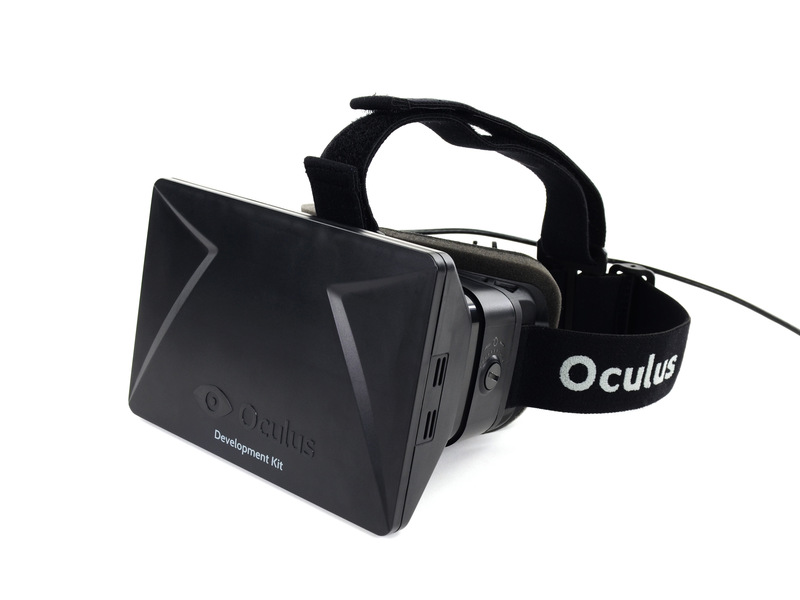
\includegraphics[width=1.0\columnwidth]{Oculus-Rift-1}
\caption{Oculus Rift}
\label{Rift}
\end{subfigure}
\begin{subfigure}{0.25\columnwidth}
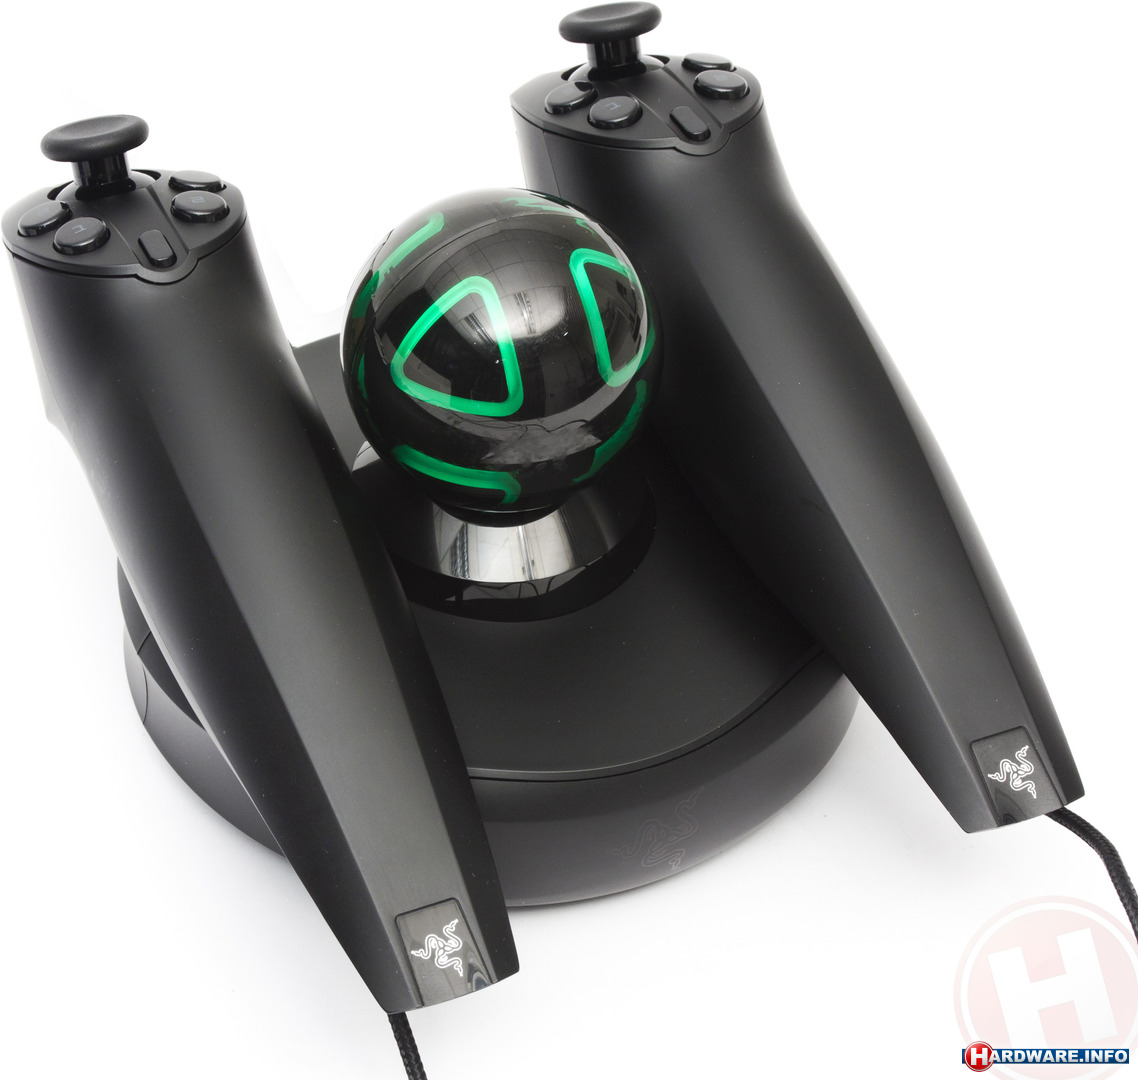
\includegraphics[width=1.0\columnwidth]{razer_hydra__portal_2}
\caption{Razer Hydra}
\label{Hydra}
\end{subfigure}
\begin{subfigure}{0.25\columnwidth}
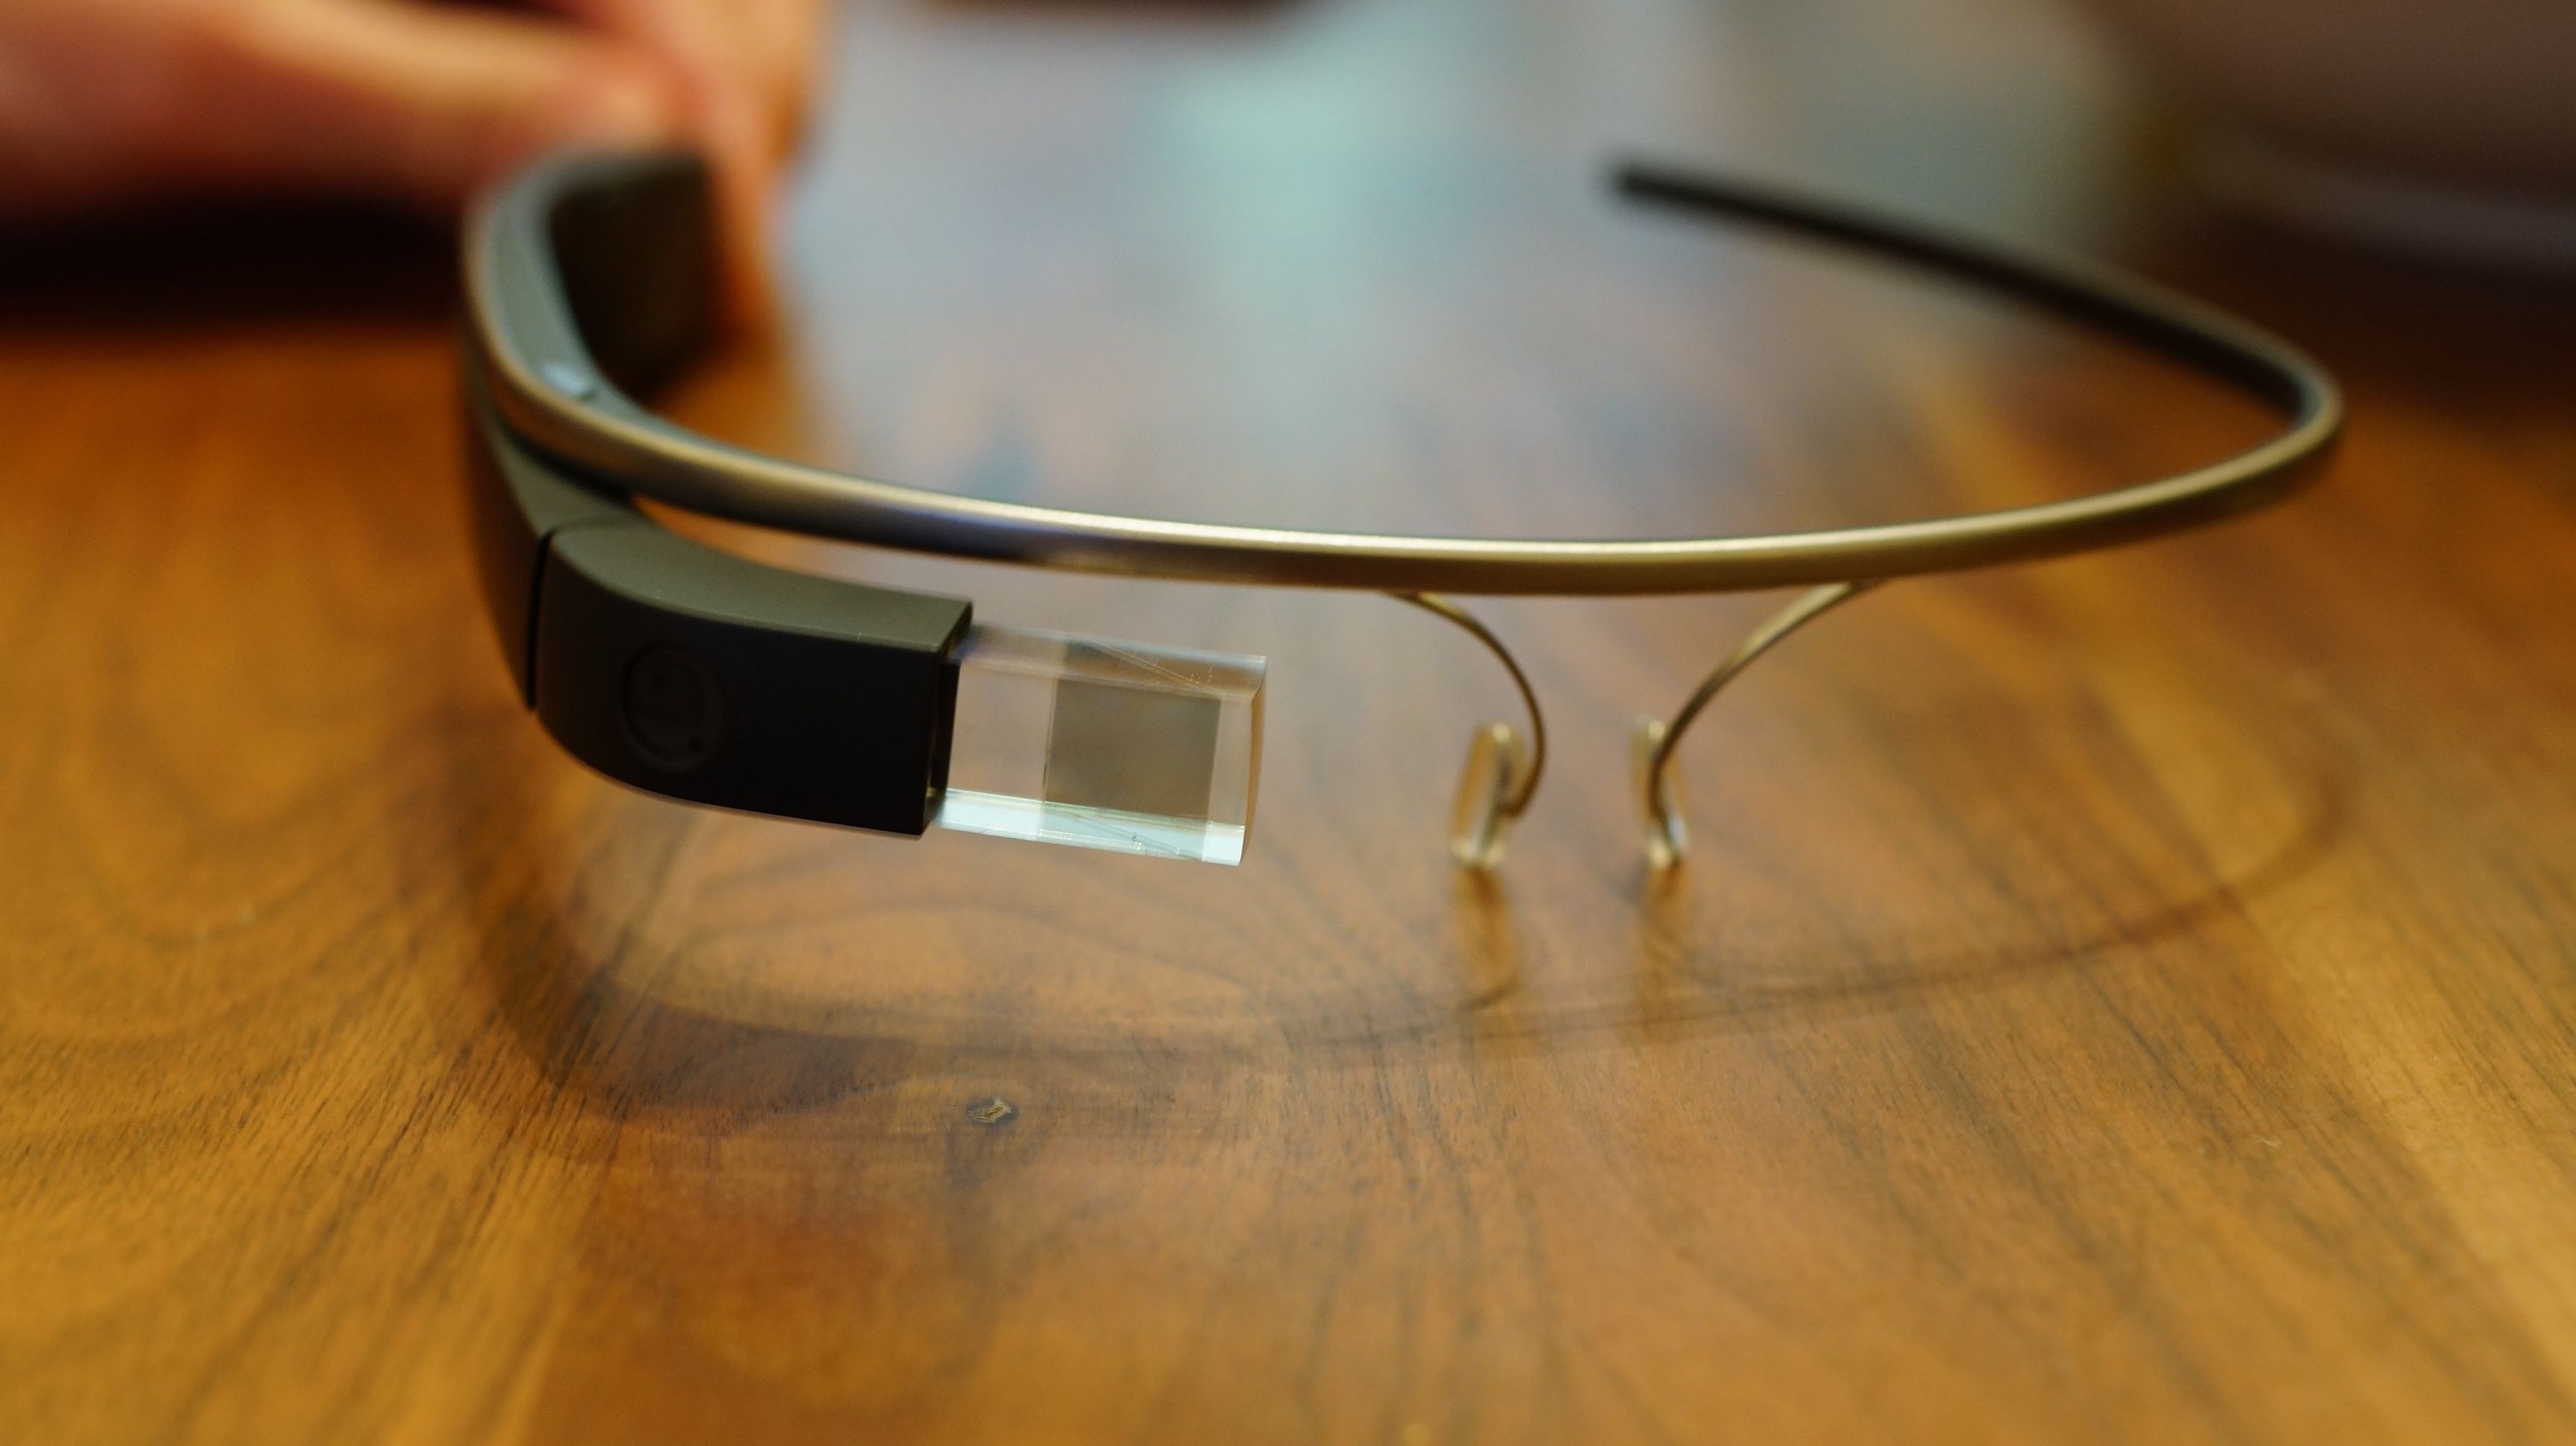
\includegraphics[width=1.0\columnwidth]{Google_Glass_Explorer_Edition}
\caption{Google Glass}
\label{Glass}
\end{subfigure}
\end{figure}

This next focus of research will involve developing a shared autonomy approach between the user, Google Glass, and the robot. The user can label objects using the Glass interface, and have that semantic mapping wirelessly sent to the robot. This semantic mapping can then be used as additional information when learning by demonstration and when giving tasks to the robot.

%For example, Google Glass can easily positively classify a desk, but it cannot know whose desk it is, or what the desk is used for. The user can tell Google Glass that this particular desk is his work desk, and when later gives a task to the robot to bring a book to his work desk, the robot will already have this semantic information.

\section{Multi-Robot Coordination}
%Final goal is multirobot interaction. RIDE was built to allow one user to control many robots directly. I want to make these tasks higher level. The user will be able to click on two robots, and right click an object. They see an interface with available actions, and the robots coordinate to accomplish that action. This is learned through a combination of demonstration and hierarchical learning (cite hierarchical learning paper. Maybe Q-MAX?).

%This can be extended to Glass. Rather than clicking on two robots, glass can be used in combination with a projector interface (Like Dan's work) for people with disabilities.

RIDE was originally created to allow one user to control many robots directly, or take a supervisory role. However, the current supervisory role can be expanded to include giving high level goals, such as bringing the user a book. Combining the abilities learned through demonstration in Section \ref{Learning by Demonstration} and the semantic information obtained during object classification in Section \ref{Object Classification}, we can build a new interface allowing users to give high level goals to a group of robots. This interface will look like a classic real time strategy game, where user gives high level commands to a large number of troops.

When using RIDE to assign tasks, the user will be able to select one or more robots, and then select an object which has been given a semantic mapping. The RIDE interface will display to the user tasks that had been learned which involve interaction with this object and the selected number of robots. The selected robots will then coordinate to accomplish the task given to them by the user. These goal-based tasks will utilize previously learned actions from Section \ref{Learning by Demonstration}. For example, we have two robots, a PR2 and Turtlebot. The PR2 is large and slow, but has limbs, while the Turltebot has no ability to interact with the environment, but is fast. Through learning by demonstration the PR2 has learned to pick up a book, and has learned to set it down, and the Turlebot has learned to move from one location to another. If the user gave these robots a task to bring a book to himself, they can coordinate these smaller tasks together to perform the larger goal. The PR2 can put the book on the Turtlebot, and the Turtlebot can delver it.

To accomplish this, each robot will know what tasks it is capable of performing and how well it performs the task. They will will be able communicate this information with each other and coordinate. The previous example required three tasks: picking up book, setting down book, and moving. The PR2 will know it is efficient at the first two tasks, but slow at the third, where the Turtlebot knows it cannot perform the first two tasks, but performs the third task well. Applying this coordination allows simple robots to be able to perform much more complicated tasks.  

\section{Conclusion}
Those suffering from ALS and quadriplegia need robots in the world now, and cannot wait for full autonomy of every task. This work intends to help those suffering from severe physical disabilities by giving them the ability to teach the robot themselves, as well as easily give positive and negative feedback. By using our shared autonomy approach we separate the low-level reactivity from the higher level reasoning, and give the higher level reasoning task to the user. 

This work also helps further the state of the art in reinforcement learning by introducing a new learning from demonstration technique that utilizes human demonstration from non-experts. This requires robots to learn from human demonstrations, even when those demonstrations are highly suboptimal. It also furthers the field in robot coordination, allowing a robot to evaluate its own performance, and utilize that information to efficiently coordinate. 
%One of the key difficulties of assistive robots is human trust. If humans had constant direct control of the robot, they would be forced to extend a high cognitive load and take a lot of time every situation they wanted the robot to perform a task. With a shared autonomy system, humans perform the high level reasoning, while the robot retains the low level reactivity.

With these new interfaces and tools, individuals with disabilities will be able to accomplish day-to-day tasks without human assistance. The lack of a human assistant performing the task and the addition of positive experiences like teaching, doing it yourself, and being more independent gets us closer to our goal of putting robots into real homes to help those with physical disabilities.

%Our first avenue of work involves extending RIDE to allow users to easily teach robots through demonstration. The two interfaces we develop will give us insight on how to design a remote learning by demonstration system for users with and without disabilities. This interface will allow users to be able to teach robots how to perform tasks around their home easily and efficiently.

%We will combine the learning by demonstration interface with a Google Glass object classification system. This Google Glass system will allow users to add semantic information to objects within their home. This semantic information can be sent to the robot wirelessly, and used when given tasks.

%Lastly, we will extend this work for multi-robot interaction. By extending RIDE to become task-based, users will be able to give high level tasks to one or many robots, applying the previously learned behavior and semantic mappings. This interface will be able to be used via Google Glass, for hands-free task allocation.




\bibliographystyle{aaai}
\bibliography{thesis}

\end{document}
